\documentclass[
    a4paper,
    dvipsnames, % more color names with xcolor
]{scrreprt}

%%% PACKAGES %%%

% PDF/A Compliance
\usepackage[a-2b,latxmp]{pdfx}
\catcode30=12

% add unicode support and use german as language
\usepackage[utf8]{inputenc}
\usepackage[ngerman]{babel}

% Use Helvetica as font
\usepackage[scaled]{helvet}
\renewcommand\familydefault{\sfdefault}
\usepackage[T1]{fontenc}

% Better tables
\usepackage{tabularx}
\usepackage{xcolor} % more colors
\usepackage{colortbl} % color cells
\usepackage{booktabs} % \midrule & \toprule & \bottomrule
\usepackage{multirow} % multi-row cells in tables

% Better enumerisation env
\usepackage{enumitem}

% Use graphics
\usepackage{graphicx}

% Have subfigures and captions
\usepackage{subcaption}

% Be able to include PDFs in the file
\usepackage{pdfpages}

% Have custom abstract heading
\usepackage{abstract}

% Need a list of equation
\usepackage{tocloft}
\usepackage{ragged2e}

% Better equation environment
\usepackage{amsmath}

% Symbols for most SI units
\usepackage{siunitx}

\usepackage{csquotes}

% clickable links to websites and chapters
\usepackage{hyperref}
\hypersetup{
  colorlinks   = true, %colours links instead of ugly boxes
  urlcolor     = RoyalPurple, %colour for external hyperlinks
  linkcolor    = Sepia, %colour of internal links
  citecolor    = Sepia, %colour of citations
  breaklinks   = true
}

% shortcut to create refrences
\newcommand*{\fullref}[1]{\hyperref[{#1}]{\ref*{#1}~``\nameref*{#1}''}}

% Change page rotation
\usepackage{pdflscape}

% Symbols like checkmark
\usepackage{amssymb}
\usepackage{pifont}

\usepackage[absolute]{textpos}

% Glossary, hyperref, babel, polyglossia, inputenc, fontenc must be loaded before this package if they are used
\usepackage{glossaries}
% Redefine the quote charachter as we are using ngerman
\GlsSetQuote{+}
% Define the usage of an acronym, Abbreviation (Abbr.), next usage: The Abbr. of ...
\setacronymstyle{long-short}

% Display CSV files as table
\usepackage{csvsimple}

% Bibliography & citing
\usepackage[
	backend=biber,
	style=apa,
	bibstyle=apa,
	citestyle=apa,
	sortlocale=de_DE
	]{biblatex}
\addbibresource{Referenzen.bib}
\DeclareLanguageMapping{ngerman}{ngerman-apa}

% Clickable Links to Websites and chapters
% From the documentation: "Make sure it comeslastof your loaded packages, to give it a fighting chance of not beingover-written, since its job is to redefine many LATEX commands"
\usepackage{hyperref}

%%% COMMAND REBINDINGS %%%
\newcommand{\tabitem}{~~\llap{\textbullet}~~}
\newcommand{\xmark}{\ding{55}}
\newcommand{\notmark}{\textbf{\textasciitilde}}
% Pro/Con item https://tex.stackexchange.com/questions/145198/change-the-bullet-of-each-item#145203
\newcommand\pro{\item[$+$]}
\newcommand\con{\item[$-$]}

%%% TRAVIS DEPENDENCY
% Can delete if you don't use Travis for CI/CD
% Fallback DocumentVersion for the preamble if built locally
\providecommand{\docversion}{0.0-localBuild}

% Define list of equations - Thanks to Charles Clayton: https://tex.stackexchange.com/a/354096
\newcommand{\listequationsname}{\huge{Formelverzeichnis}}
\newlistof{myequations}{equ}{\listequationsname}
\newcommand{\myequations}[1]{
	\addcontentsline{equ}{myequations}{\protect\numberline{\theequation}#1}
}
\setlength{\cftmyequationsnumwidth}{2.3em}
\setlength{\cftmyequationsindent}{1.5em}

% Usage {equation}{caption}{label}
% \indexequation{b = \frac{\pi}{\SI{180}{\degree}}\cdot\beta\cdot 6378.137}{Bogenlänge $b$ des Winkels $\beta$ mit Radius 6378.137m (Distanz zum Erdmittelpunkt am Äquator)}{Bogenlaenge}
\newcommand{\indexequation}[3]{
	\begin{align} \label{#3} \ensuremath{\boxed{#1}} \end{align}
	\myequations{#3} \centering \small \textit{#2} \normalsize \justify }

% Todolist - credit to https://tex.stackexchange.com/questions/247681/how-to-create-checkbox-todo-list
\newlist{todolist}{itemize}{1}
\setlist[todolist]{label=$\square$}

% Nested Enumeratelist credit to https://tex.stackexchange.com/a/54676
\newlist{legal}{enumerate}{10}
\setlist[legal]{label*=\arabic*.}

%%% PATH DEFINITIONS %%%
% Define the path were images are found
\graphicspath{{./img/}{./appendix/}}

%%% GLOSSARY ENTRIES %%%
\makeglossaries
% \newacronym{RFID}{RFID}{Radio-Frequency Identification}
% \newglossaryentry{HF}{name={HF},description={High Frequency, RFID Tags im Frequenzbereich von 3-30MHz}}


%%% DOCUMENT %%%

\begin{document}

% !TEX root = BA-Bericht.tex
\begin{titlepage}
	\begin{textblock*}{5cm}[0,0](15.1cm,0.7cm)
		
\includegraphics[keepaspectratio,width=5cm]{img/HSLU_Logo}
	\end{textblock*}
	\begin{center}
		\vspace*{5cm}
        \Huge{Untersuchung der Performance des Invisible Internet Protocols (I2P)\textbf{}} \\
		\Large{Ist ein grösseres Netzwerk performanter?}\\
		\vspace{0.5em}
		\Large{Bachelorarbeit FS2021}\\
		\vspace{3em}
		\LARGE{Studentin / Student}\\
		\LARGE{Moritz Küttel}\\
		\vspace{1em}
		\Large{Betreuer:}\\
        \large{Dieter Arnold}
		\vfill
		\large{Hochschule Luzern - Departement Informatik}\\
		\large{\today}\\
		\large{Version \docversion}
	\end{center}
	\begin{textblock*}{5cm}[0,0](15.3cm,277mm)
		
\includegraphics[keepaspectratio,width=5cm]{img/FHZ_Logo}
	\end{textblock*}
\end{titlepage}

\newpage

\pagenumbering{gobble}

\begin{textblock*}{5cm}[0,0](15cm,0.7cm)
	
\includegraphics[keepaspectratio,width=2.7cm]{img/HSLU_Logo_Header}
\end{textblock*}

\vspace*{1.35cm}

\fontsize{12}{14}
\textbf{Bachelorarbeit an der Hochschule Luzern -- Informatik} \\ \vspace*{0.6cm}

\fontsize{10.5}{12}
\noindent
\textbf{Titel:} Untersuchung der Performance des Invisible Internet Protocols (I2P)\newline \newline
%TODO: HSLU Preamble titel
\textbf{Studentin/Student:} Moritz Küttel \newline \newline
\textbf{Studentin/Student:} - \newline \newline
\textbf{Studiengang:} BSc Informatik oder Wirtschaftsinformatik \newline \newline
\textbf{Jahr:} 2021\newline \newline
\textbf{Betreuungsperson:} Dieter Arnold \newline \newline
\textbf{Expertin/Experte:} Urs Rufer \newline \newline
\textbf{Auftraggeberin/Auftraggeber:} Carolyn Bächler, Konrad Bächler\newline \newline \newline
\textbf{Codierung / Klassifizierung der Arbeit:}\\
$\square$ A: Einsicht   (Normalfall) \\
$\square$ B: R\"ucksprache      (Dauer:  \ \ \ \ \     Jahr / Jahre)\\
$\square$ C: Sperre     (Dauer:  \ \ \ \ \     Jahr / Jahre)\\


%%% you can use \boxtimes for filling a cross inside the square
%%% e.g., $\boxtimes$ A: Einsicht       (Normalfall)


\paragraph{\textbf{Eidesstattliche Erkl\"arung}}
Ich erkl\"are hiermit, dass ich/wir die vorliegende Arbeit selbst\"andig und ohne unerlaubte fremde Hilfe angefertigt haben, alle verwendeten Quellen, Literatur und andere Hilfsmittel angegeben haben, w\"ortlich oder inhaltlich entnommene Stellen als solche kenntlich gemacht haben, das Vertraulichkeitsinteresse des Auftraggebers wahren und die Urheberrechtsbestimmungen der Fachhochschule Zentralschweiz (siehe Merkblatt <<Studentische Arbeiten>> auf MyCampus) respektieren werden. \newline \newline
Ort / Datum, Unterschrift       \underline{\hspace*{4cm}} \newline \newline
Ort / Datum, Unterschrift       \underline{\hspace*{4cm}}


\newpage
\noindent
\textbf{Abgabe der Arbeit auf der Portfolio Datenbank:}\\
Best\"atigungsvisum Studentin/Student\\
Ich best\"atige, dass ich die Bachelorarbeit korrekt gem\"ass Merkblatt auf der Portfolio Datenbank abgelegt habe. Die Verantwortlichkeit sowie die Berechtigungen habe ich abgegeben, so dass ich keine \"Anderungen mehr vornehmen kann oder weitere Dateien hochladen kann. \newline \newline
Ort / Datum, Unterschrift       \underline{\hspace*{4cm}} \newline \newline
Ort / Datum, Unterschrift   \underline{\hspace*{4cm}} \newline \newline \newline
\textbf{Verdankung}\\
{\color{red}TODO Write verdankung} \newline \newline \newline
\noindent
{\textbf{Ausschliesslich bei Abgabe in gedruckter Form: \\
Eingangsvisum durch das Sekretariat auszuf\"ullen}} \newline \newline
Rotkreuz, den   \underline{\hspace*{4cm}} \hspace*{1cm} Visum:  \underline{\hspace*{4cm}} \vspace*{10cm}


\noindent
{\textbf{Hinweis}}: Die Bachelorarbeit wurde von keinem Dozierenden nachbearbeitet. Ver\"offentlichungen (auch auszugsweise) sind ohne das Einverst\"andnis der Studiengangleitung der Hochschule Luzern -- Informatik nicht erlaubt. \newline \newline
Copyright \textcopyright\ {\color{red}2019} Hochschule Luzern -- Informatik \newline \newline
Alle Rechte vorbehalten. Kein Teil dieser Arbeit darf ohne die schriftliche Genehmigung der Studiengangleitung der Hochschule Luzern -- Informatik in irgendeiner Form reproduziert oder in eine von Maschinen verwendete Sprache \"ubertragen werden.

\begin{textblock*}{5cm}[0,0](14.93cm,277mm)
	
\includegraphics[keepaspectratio,width=5cm]{img/FHZ_Logo}
\end{textblock*}

\newpage
\pagenumbering{arabic}



\pagenumbering{Roman}

\begin{abstract}
	% TODO Abstract schreiben =)
\end{abstract}

\tableofcontents

\clearpage
\pagenumbering{arabic}

% !TEX root = BA-Bericht.tex
\chapter{Einleitung}
\label{ch:Einleitung}
% TODO Allgemeine Einleitung in die Arbeit

In der heutigen hochvernetzten und globalisierten Welt von Big-Data scheinen die Thematiken Datenschutz und Privatsphäre oft unterzugehen.

Das Internet Protokoll (IP) ist eines der Grundsteine für das heutige Internet.
Dieses wurde jedoch damals unter nicht den gesichtspunkten wie Datenschutz, Privatsphäre und Sicherheit designt.
Es ging wohl eher darum, dass überhaupt ein Protokoll da war, um Nachrichten in einem Netzwerk zu routen.

Mittlerweile gibt es jedoch verschiedene Anonymisierungsnetzwerke, welche in diesem Bereich abhilfe schaffen könnten.

Die Performance dieser Netzwerke ist jedoch aber nie so gut wie von IP direkt. (siehe Anonymitätstrilemma).
Für Benutzer lässt die Performance jedoch oft zu wünschen übrig.
Auch sonst gibt es für Benutzer nicht wirklich Argumente wieso, solch ein Netzwerk eingesetzt werden soll, da es kaum Anwendungen gibt.


\section{Aufgabenstellung}

Das freie Software- und Netzwerkprojekt DIVA.EXCHANGE\footnote{Webauftritt: \url{https://diva.exchange}} entwickelt einen Softwareprototypen DIVA.
Der Softwareprototyp soll aufzeigen, dass es möglich ist eine sichere und dezentrale Handelsplattform für digitale Werte zu erstellen, welche auch die Privatsphäre der Benutzer schützt.

Der Softwareprototyp besteht aus drei Schichten.
Einer Anonymisierungsschicht auf Netzwerkebene (\glsname{i2p}), einer Datenhaltunsschicht basierend auf einer Blockchain und eine darüberliegende Handels- und Verwaltungssoftware.

Siehe auch die komplette Aufgabenstellung im Anhang \fullref{ch:aufgabenstellung}.

\section{Problem}

Es besteht die Annahme, dass die Performance des \glsname{i2p}-Netzwerk's nicht ausreichend ist, um für Endbenutzer schnell reagierende Applikationen auf dem Netzwerk anbieten zu können.
Kurz vor Beginn dieser Arbeit dauerte das Hin- und Zurücksenden einer Nachricht durch das \glsname{i2p}-Netzwerk (Roundtrip) etwa drei bis acht Sekunden.

Das Netzwerk ist verglichen mit dem \glsname{tor} klein und es können grössere Latenzen entstehen, um Anonymität für die Teilnehmer zu bieten:

\begin{itemize}
    \item Eine Nachricht wird über mehrere Hops versendet und wird mehrmals weitergeleitet bevor diese bei ihrem Ziel ankommt.
    \item Fallen Hops aus müssen die Nachrichten neu über eine andere Route übermittelt werden.
    \item Jede Nachricht ist mehrfach verschlüsselt und jeder Knoten muss jeweils eine Verschlüsselungsschicht beim weiterleiten einer Nachricht entfernen was viele CPU-Zyklen kostet.
\end{itemize}


\section{Fragestellung}

Im Rahmen dieses Projekts soll folgende Problemstellung erarbeitet werden:

\begin{hyp}[H\ref{hyp:first}] \label{hyp:first}
    Ist eine steigende Anzahl von I2P-Knoten für die I2P-Netzwerk-Latenz (tiefer) vorteilhaft?
    Können Nachrichten schneller vom Sender zum Empfänger gelangen je mehr Knoten das I2P-Netzwerk hat?
\end{hyp}

\begin{hyp}[H\ref{hyp:second}] \label{hyp:second}
    Führt eine steigende Anzahl von I2P-Knoten für eine Vergrösserung der I2P-Netzwerk-Bandbreite?
\end{hyp}

\begin{hyp}[H\ref{hyp:third}] \label{hyp:third}
    Führt eine grössere Anzahl an Verbindungen zwischen den I2P-Knoten zu einer Verringerung der Latenz?
\end{hyp}

\begin{hyp}[H\ref{hyp:fourth}] \label{hyp:fourth}
    Führt eine grössere Anzahl an Verbindungen zwischen den I2P-Knoten zu einer Vergrösserung der I2P-Netzwerk-Bandbreite?
\end{hyp}

Damit Applikationen auf dem I2P-Netzwerk gut funktionieren, soll ermittelt werden wie die Performance
verbessert werden soll.

\section{Vorgehen und Methode}


Es soll ein iteratives Projektmanagement verwendet werden
Zum überprüfen der Hypothese sollen Experimente/Sim

\section{Ziel}

Es gilt aufzuzeigen unter welchen Umständen und Rahmenbedingungen Anwendungen auf dem \glsname{i2p}-Netzwerk kürzere Latenzzeiten aufweisen
und somit für Endbenutzer schneller reagieren können. Das Niveau an Anonymität soll aber beibehalten bleiben.


\section{Vision}

Wird festgestellt, dass mehr Knoten in einem I2P-Netzwerk die Latenz verringert.
Diese Erkenntnis könnte auch unter Umständen mehr Personen dazu bewegen selber \glsname{i2p}-Knoten zu betreiben.
Dies wiederum würde das Netzwerk stärken und diverse Netzwerkeffekte könnten auftreten.
Zum Beispiel könnte dies dazu führen, das mehr Entwickler Applikationen für das Netzwerk erstellen und es auch aus Benutzerseite attraktiver wird.

% Welche Ziele, Fragestellungen werden mit dem Projekt verfolgt? Die Bedeutung, Auswirkung und
% Relevanz dieses Projektes für die unterschiedlichen Beteiligten soll aufgeführt werden.
% Typischerweise wird hier ein Verweis auf die Aufgabenstellung im Anhang gemacht.

\section{Struktur des Berichts}
% outline the order of information in the thesis

Im nächsten Kapitel~\fullref{ch:standdertechnik} ....

Im Kapitel~\fullref{ch:methode} wird beschrieben welche Methoden .... 



\chapter{Stand der Technik}
\label{ch:StandDerTechnik}
% Auch "Stand der Forschung" oder "Stand der Praxis"

% Bezogen auf die eigenen Zielsetzungen und Fragestellungen soll aufgezeigt werden, wie andere
% dieses oder ähnliche Probleme gelöst haben. Worauf können Sie aufbauen, was müssen Sie neu
% angehen? Wodurch unterscheidet sich Ihre Lösung von anderen Lösungen? Für wissenschaftlich
% orientierte Arbeiten sei hier explizit auf (Balzert, S. 66 ff) verwiesen.

% TODO Historie des betroffenen Feld

\section{Technologische Grundlagen}
% TODO Wichtige technologischen Grundlagen / Wissenswertes

\subsection{I2P}

I2P ist ein \glsname{p2p}-Netzwerk.


\cite{astolfi_i2p_2015}

\subsection{Wie I2P funktioniert}

\section{Technische Konzepte}
\label{sec:technischeKonzepte}
% TODO Konzepte in diesem Feld welche für den Leser relevant sind

\section{Stand im Bezug auf eigenes Projekt}
% TODO Welche Forschung wurde in jüngster Zeit gemacht welche relevant für das eigene Projekt sind


\chapter{Ideen und Konzepte}

Dieses Kapitel soll aufzeigen wie ein Teststand erstellt werden soll um die Performance eines I2P-Netzwerkes zu messen. Es wird ein Konzept für einen Testand vorgestellt der den Anforderungen (siehe Abschnitt~\ref{sec:Anforderungen}) gerecht werden soll.

Angefangen mit dem Abschnitt \ref{sec:grundidee} werden verschiedene Lösungsansätze für verschieden Aspekte vorgestellt.

\section{Grundidee}\label{sec:grundidee}
% TODO Beschreibung wie das Problem im Ansatz gelöst werden soll

% Hier geht es um die Fragestellung, wie Sie die formulierten Ziele der Arbeit erreichen wollen.
% Sie halten z.B. erste, grobe Ideen, skizzenhafte Lösungsansätze fest. Gibt es mehrere Wege, Ansätze
% um dieses Ziel zu erreichen, begründen Sie hier, warum Sie einen bestimmten Weg einschlagen.
% Beispiel für ein Softwareprojekt: Erste Gedanken über eine grobe Systemarchitektur. Ist z.B. eine
% Microservice-Architektur angebracht? Welche Alternativen bestehen, wo gibt es Problempunkte? Die
% Umsetzung, die Beurteilung der Machbarkeit und die detaillierte Beschreibung der umgesetzten
% Architektur sind dann Teil der Realisierung.

% Abgrenzung zu Kapitel 5 (Realisierung):
% - Besteht ein wesentliches Projektziel darin, für Ihre Kunden z.B. ein Security-Konzept, ein
% Kommunikations-Konzeptes, ein IT-Fachkonzept oder ein anderes Fach-Konzept zu erstellen, dann
% wird die Entwicklung dieser (fachlichen) Konzepte unter «Realisierung» beschrieben (sie sind ja der
% eigentliche Kern Ihrer Arbeit).
% - Besteht z.B. ein wesentliches Ziel der Arbeit darin, eine passende Software-Architektur zu
% evaluieren, dann gehören die entsprechenden Beschreibungen ins Kapitel 5.

Grundsätzlich soll ein Teststand aufgebaut werden an dem empirische Performance Messungen an einem I2P-Testnetzwerk durchgeführt werden können \seereq{TINF}.
Dabei gibt es verschiedene Herausforderungen und Aspekte die es zu beachten gilt.


\section{Reproduzierbarkeit}

Um ein Test auf einem solchen Testnetzwerk wiederholbar und reproduzierbar zu machen gibt es folgendes zu beachten \seereq{TREP}.

\begin{itemize}
    \item Das Testnetzwerk soll isoliert werden um äussere einflüsse durch das Netzwerk (auch das offizielle I2P Netzwerk) zu vermeiden (siehe auch Abschnitt~\ref{sec:isolierung}).
    \item Infrastructure as Code: Ist die Testinfrastruktur als Programmcode beschrieben, kann dieser zu einem späteren Zeitpunkt wieder ausgeführt werden, um das Testnetzwerk wieder zu erstellen. Mehr dazu im Abschnitt~\ref{sec:deployment}.
    \item Reproduzierbarer Build von \lstinline|i2pd| und der Software auf einem Knoten
\end{itemize}

Dies könnte mit verschiedenen Tools gelöst werden. Nix könnte hier insbesondere hilfreich werden, da reproduzierbare builds, wie auch mit nixops ein ''Infrastructure as Code''-Tool angeboten wird.

\section{Deployment}\label{sec:deployment}

Wichtig für das Deployment ist das schnell neue Tests gestartet und neue Testnetzwerke erstellt werden \seereq{TPER}.
Und dies mit verschiedenen Konfigurationen \seereq{TCNF}.
Die im Vorherigen Abschnitt bereits erwähnt soll das Deployment auch reproduzierbar sein \seereq{TREP}.
Es soll auch möglich sein verschieden grosse Testnetzwerke zu erstellen \seereq{TSCL}.



\subsection{Container oder Virtuelle Maschinen}

Um Ressourcen zu schonen aufgrund von kleinerem Overhead und Start-Up-Time von Containern im Gegensatz zu VMs sind diese wohl zu bevorzugen.
Container erlauben es schneller tests durchzuführen \seereq{TPER} aufgrund der Start-Up/Deployment-Time
aber auch Tests mit mehr Knoten zu machen, da weniger Ressoucen für einen einzellnen Knoten benötigt wird.
Dies ist der Fall weil bei Containerlösungen (oder auch OS-Virtualisierung) im Gegensatz zu Virtuellen Maschinen der Betriebsystemkernel zwischen den Instanzen geteilt wird.

\subsection{Bootstrapping}

Ganz zu Beginn, wenn ein Knoten dem I2P Netzwerk beitritt muss dieser Wissen wo mindestens ein anderer Knoten ist.
Um die erste Liste von Knoten zu erhalten damit Knoten dem Netzwerk beitreten können, muss die liste von Knoten im Netzwerk zu beginn des Tests ''geseedet'' werden. TODO: Explain this better

\subsection{Tools}

Es gibt verschiedene Tools für deployment von Netzwerken wie z.B. \lstinline|docker-compose|, \lstinline|kubernetes|, \lstinline|terraform|, oder auch \lstinline|nixops|.


\section{Konfigurierbarkeit}

Folgendes soll im Teststand konfigurierbar sein (\reqref{TCNF}):

\begin{itemize}
    \item Anzahl Knoten
    \item Maximale Bandbreite
    \item Hops (länge der Tunnel)
    \item In welchem Netzwerk (familiy netzwerk/öffentliches Netzwerk) (für Vergleich/optional)
\end{itemize}

Nix als konfigurationssprache würde es erlauben beliebige aspekte des Setups konfigurierbar zu machen.
Die meisten oben erwähnten Konfigurationsmöglichkeiten werden bereits durch verschiedene NixOS-Module (\lstinline|i2pd|, \lstinline|firewall|, ... ) angeboten.

\section{Latenzmessung von Nachrichten}

Um die Latenz oder Verzögerung einer Nachricht im Testnetzwerks zu messen \seereq{TLAT}, könnte man jeweils den Empfangs- sowie Sendezeitpunkt einer Nachricht speichern und voneinander subtrahieren.
Jedoch muss so sichergestellt werden, dass die Uhrzeiten zwischen allen Knoten synchron ist.
Dies ist jedoch ein komplexes und bekanntes Problem mit verteilten Systemen.
Je nach dem muss eventuell auf Lamport-Zeitstempel zurückgegriffen werden?

\section{Limitieren der Bandbreite}

\lstinline|i2pd|
erlaubt es die Bandbreite eines Knotens \seereq{TLIM} mittels der \lstinline|bandwidth| Konfigurationseinstellung \seereq{TCNF} zu limitieren.

\begin{itemize}
    \item Die Bandbreite eines i2pd Knoten kann limitiert werden in der Konfiguration mit der Einstellung bandwidth.  
    \item \cite{noauthor_i2p_nodate-3}
    \item Tc - Traffic control tool
    \item Nix Tooling
\end{itemize}

\section{Isolierung des Testnetzwerks}
\label{sec:isolierung}

Das Diagramm~\fullref{fig:i2p-testnetwork} zeigt den Aufbau des Testnetzwerks auf. Das Testnetzwerk soll standardmässig weder mit dem Internet verbunden noch mit dem System des Testers, um äussere Einflüsse zu verringern und durch isolation bessere Reproduzierbarkeit zu erreichen.

\begin{figure*}[ht]
  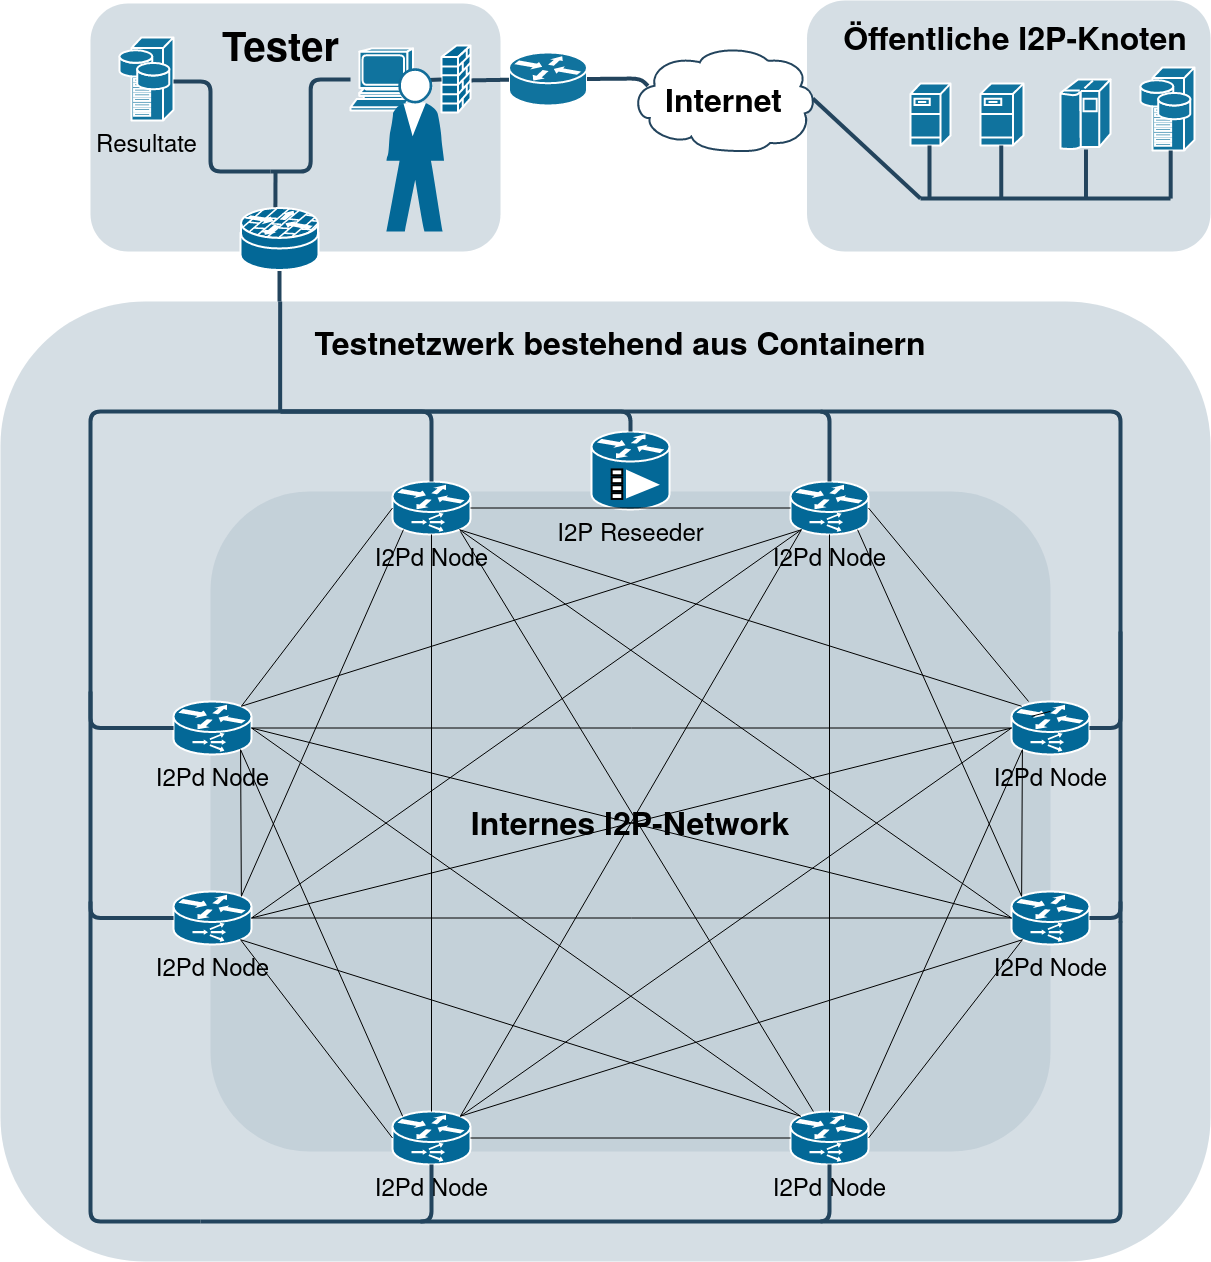
\includegraphics[width=1.0\textwidth]{i2p-testnetwork.png}
  \caption{I2P Testnetwork}\label{fig:i2p-testnetwork}
\end{figure*}

Bei der Firewall handelt es sich entweder um das Hostsystem (VM-Network) für das Testnetzwerk selber, welche die i2p-Knoten hostet, oder um einen extra Container der aller outgoing traffic kontrolliert.
Wichtig ist das der Tester, welcher das Netzwerk erstellt und die Tests durchführt sich auch ausserhalb des Testnetzwerkes befindet, um ungewollte Einflüsse zu vermeiden.

Die I2P-Knoten sind als Router dargestellt und befinden sich eigentlich alle in zwei Netzwerken gleichzeitig. Das normale IP Netzwerk und das I2P-Netzwerk.

Am Ende des Tests müssen die Testresultate an einem sicheren Ort ausserhalb des Testnetzwerks abgelegt werden, damit diese später analysiert werden können. (Resul tDB)

In der \lstinline|i2pd| Konfiguration gibt es zusätzlich das \lstinline|familiy| tag, welches die Knoten als zusammenhängend markieren würde, würden diese aus Versehen mit dem echten I2P Netzwerk reden. Dies ist auch interessant bezüglich Tests die am echten Netzwerk durchgeführt werden sollen.

TODO: Verschiedene Netzwerksegmente mit verschiedenen Knoten?

\section{Messen der Ressourcenauslastung der Knoten}

Die Messung der Ressourcenauslastung der Knoten könnte sinnvoll sein aus mehreren Gründen.
Gerät ein Knoten oder die Hostsysteme für das Testnetzwerk in Ressourcenengpässe beeinflusst dies wahrscheinlich auch die Resultate.

\begin{itemize}
    \item Somit kann sichergestellt werden, dass das Testnetzwerk nicht so gross skaliert wurde, bzw. wie weit es skaliert werden kann \seereq{TSCL}.
    \item Um sicherzustellen das ein Flaschenhals im Netzwerk nicht durch zu wenig ressourcen verursacht sind \seereq{TPER}.
    \item Äussere einflüsse wie Ressource-Exhaustion vermeiden, dies verbessert auch die Reproduzierbarkeit \seereq{TREP}.
    \item Messung der Test-Performance
\end{itemize}

Gemessen werden sollte:

\begin{itemize}
    \item Netzwerkbandbreite (kbits/sec)
    \item CPU gebrauch (in Prozent)
    \item RAM Verwendung (in Prozent)
    \item Disk I/O (read/write, kbits/sec)
    \item Freier Speicherplatz
\end{itemize}


\chapter{Methode}
% TODO Nach eigenen Bedürfnissen erweitern
% ------------------------------------- TEIL Wissenschaftliche Arbeiten ----------------------------------------------------
\subsection{Quantitative/Qualitative Querschnittsanalyse}

\subsection{Fallstudie}

\subsection{Labor-/Feldexperiment}

% ------------------------------------- TEIL Ingenieurlastige Arbeiten ----------------------------------------------------
\section{Projektinformationen}

In diesem Abschnitt wird aufgezeigt welches Vorgehensmodell und welche Methoden verwendet wurden zur Abwicklung dieses Projektes.
Auch wird aufgezeigt wie das Projekt organisiert ist.

\subsection{Vorgehensmodell}

% TODO: vorgehensmodell festsetzen
% SoDa? KanBan? Quellen?


\subsection{Projektteam}

Die folgende Tabelle~\ref{tab:projectmembers} listet alle Personen auf die an diesem Projekt beteiligt sind.

\begin{table}[H]
    \begin{tabular}{l p{3.2cm}}
        \toprule
        \bfseries Person   & \bfseries Rollen \\
        \midrule
        Konrad Bächler     & Auftraggeber \\
        \midrule
        Carolyn Bächler    & Auftraggeber \\
        \midrule
        Arnold Dieter      & Betreuungsperson \\
        \midrule
        tbd.               & Experte \\
        % TODO: find out who's the expert
        \midrule
        Moritz Küttel      & Student \\
        \bottomrule
    \end{tabular}
    \caption{People involved in the project}\label{tab:projectmembers}
\end{table}

\subsection{Quellcode}

Der \LaTeX-Quellcode für diesen Bericht ist auf codeberg.org in diesem Repository zu finden:
\url{https://codeberg.org/mkuettel/ba}

%TODO: add links to all the source code

\subsection{Projektboard und Issue-Tracker}

Die Abbildung~\ref{fig:projectboard} zeigt das Projektboard, welches für Projektmanagement und Controlling verwendet wird.
Jede Karte auf dem Projektboard ist ein Issue aus dem Issue-Tracker:

\url{https://codeberg.org/mkuettel/ba/issues}

Der Issue-Tracker ist zugleich ein Backlog. Issues können nach Bedarf aus dem BackLog entnommen werden und zum Projektboard hinzugefügt werden.

Das Projektboard ist ein KanBan-Board und enthält drei Spalten: ''To Do'', ''In Progress'' und ''Done''.
Diese Issues aus dem Issue-Tracker können dann je nach fortschritt in die Spalten einsortiert werden. 
Ziel von KanBan ist es eines nach dem anderen zu machen und sich auf einen Task zu fokussieren. Man sollte also nie mehr als einen Issue in der Spalte ''In Progress'' haben.
%TODO: definition of done
% https://de.wikipedia.org/wiki/Kanban_(Softwareentwicklung)

%TODO: describe how issues are categorized (labels, milestones, projects etc.)

Das KanBan-Board ist hier zu finden:

\url{https://codeberg.org/mkuettel/BA/projects/125}


\begin{figure*}[ht]
    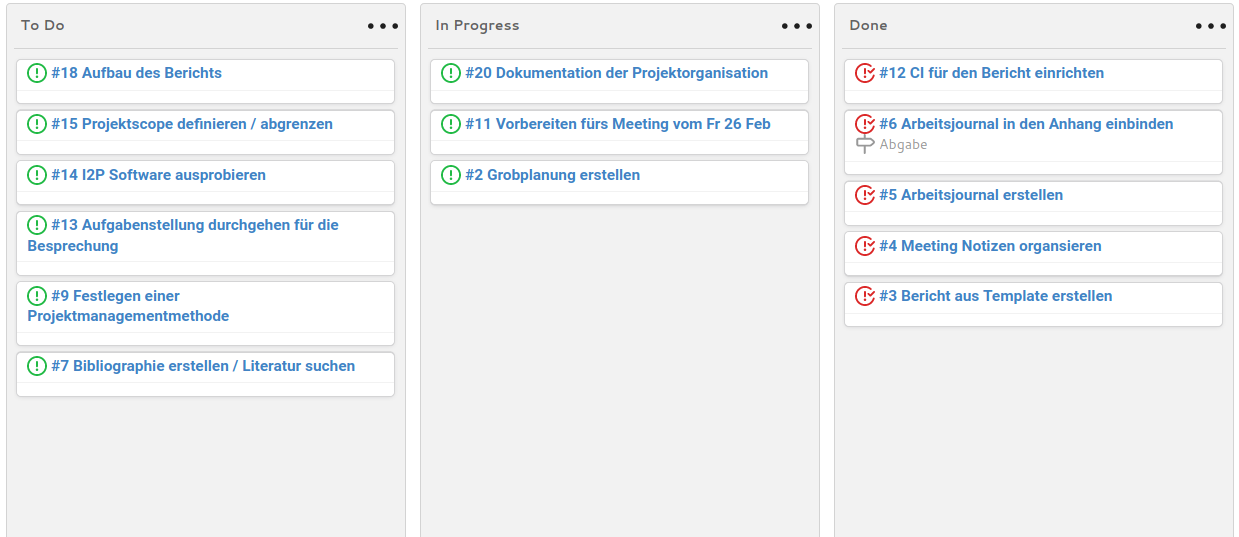
\includegraphics[width=1.0\textwidth]{project-board.png}
    \caption{CodeBerg Project Board}
    \label{fig:projectboard}
\end{figure*}


Ein einziger Issue sollte nie mehr Aufwand machen als acht Stunden Arbeit. Diese Regel hilft die Issues kleiner zu halten und genauere Aussagen treffen zu können, wo man im Projekt steht.

Wird an einem Issue gearbeitet wird dies im Journal vermerkt \& in der Git-Historie hinterlegt.
Das Arbeitsjournal ist im Anhang~\ref{sec:journal} zu finden.


Die Länge eines Sprints in KanBan ist nicht genau definiert, sondern der Sprint ist fertig wenn alle Arbeit für den jeweiligen Sprint erledigt wurde.

\subsection{Ermittlung offener Projektrahmenbedingungen}
\label{ch:evaluation}

% TODO: Requirements engineering Methode

\subsection{Projektanforderungen / Anforderungsanalyse}
\label{sub:Anforderungen}

\subsection{Einschränkungen und Abgrenzungen}

% TODO: Scope in der Einleitung
% TODO: Scope definieren

\subsection{Systemarchitektur}

\subsection{Komponentendesign}

\subsection{Umsetzung / Programmierung}

\subsection{Testing}


% !TEX root = BA-Bericht.tex
\chapter{Realisierung}
% TODO Beschreibung der Umsetzung der definierten Ziele, einschliesslich der aufgetretenen Schwierigkeiten und Einschränkungen

% Dies ist das Hauptkapitel Ihrer Arbeit! Hier wird die Umsetzung der eigenen Ideen und Konzepte
% (Kapitel 3) anhand der gewählten Methoden (Kapitel 4) beschrieben, inkl. der dabei aufgetretenen
% Schwierigkeiten und Einschränkungen.

\section{Projektmanagement}

\subsection{Meilenstein 1: Grobkonzept}

\subsection{Meilenstein 2: Zwischenpräsentation}

\subsection{Resultate}

Die folgende Tabelle~\fullref{tab:resultate} beschreibt alle Resultate und Unterresultate die während dieser Bachelorarbeit erstellt werden.
Diese Tabelle wurde zusammengestellt anhand der Anforderungen im Abschnitt~\ref{sec:Anforderungen}.

Jedes Resultat hat einen eindeutigen Identifier in  der Spalte ''Nr'' aufgelistet.
Die Spalte ``Anforderung'' bezieht sich darauf, welche Anforderungen für das jeweilige Resultat massgebend sind.
In der letzten Spalte ''Geschätzter Arbeitsaufwand'', wurde zu beginn des Projekts abgeschätzt wie viel Arbeitsaufwand (in Stunden) das Resultat verursacht.

\begin{longtable}{p{0.8cm} l p{3.5cm} p{2cm}}
    \toprule
    \bfseries Nr & \bfseries Resultat & \bfseries Anforderung& \multicolumn{1}{p{3cm}}{\bfseries Geschätzter Arbeitsaufwand} \\
    \midrule \endhead
    D            & \textbf{Dokumentation}                                       & \reqref{DOCS} & \textbf{Total 44h}  \\
    \midrule                                                               
    D.1          & \; Dokumenten Layout                                &       & 8h   \\
    D.2          & \; Aufbau des Berichts                              &       & 4h   \\
    D.3          & \; Titelseite                                       &       & 2h   \\
    D.4          & \; Zusammenfassung / Abstract                       &       & 2h   \\
    D.5          & \; Einleitung                                       &       & 4h   \\
    D.6          & \; Beschreibung Motivation / Problem                &       & 2h   \\
    D.7          & \; Beschreibung der Aufgabenstellung                &       & 2h   \\
    D.8          & \; Beschreibung der Ziele / Vision                  &       & 1h   \\
    D.9          & \; Fragestellungen / Hypothesen                     &       & 2h   \\
    D.11         & \; Reflektion / Fazit                               &       & 3h   \\
    D.12         & \; Persönliches Projektfazit                        &       & 1h   \\
    D.13         & \; Ausblick                                         &       & 4h   \\
    D.14         & \; Anhang                                           &       & 3h   \\
    D.15         & \; Zwischenpräsentation                             & \reqref{PRES}  & 6h  \\
    \midrule                                                               
    R            & \textbf{Research State of the Art}                           & \reqref{SDTF} \reqref{DOCS}  & \textbf{Total 40h} \\
    \midrule                                                               
    R.1          & \; Literatur sammeln (Recherche)                    &       & 12h  \\
    R.2          & \; Bibliographie erstellen                          &       &  4h  \\
    R.3          & \; P2P Networks                                     &       &  2h  \\
    R.3.1        & \;   - Latenz / Bandbreite / Performanz             &       &  2h  \\
    R.4          & \; Beschreibung I2P                                 &       & 10h  \\
    R.4.1        & \; -- Begrifflichkeiten                              &       &  4h  \\
    R.4.2        & \; -- Funktionsweise                                 &       &  2h  \\
    R.4.3        & \; -- Bandbreite                                     &       &  2h  \\
    R.4.4        & \; -- Latenz                                         &       &  2h  \\
    R.5          & \; Deployment von Testnetzwerken                    &       &  4h  \\
    R.6          & \; Beschreibung der Wissenschaftlichen Methode      &       &  2h  \\
    R.7          & \; Metriken für die Auswertung                      & \reqref{TPER} \reqref{TISO} \reqref{TREP}  &  6h  \\
    \midrule                                                               
    K            & \textbf{Testkonzept          }                               & \reqref{TKON} \reqref{DOCS}  & \textbf{Total 46h}  \\
    \midrule                                                               
    K.1          & \; Beschreibung Ideen / Konzepte                    &       &  4h  \\
    K.2          & \; Anforderungen an den Teststand                   &       &  4h  \\
    K.3          & \; Teststrategie                                    &       &  4h  \\
    K.4          & \; Architektur Teststand                            &       &  4h  \\
    K.5          & \; Komponentendiagramm                              &       &  2h  \\
    K.6          & \; Beschreibung was gemessen werden soll            &       &  8h  \\
    K.7.1        & \; -- Bandbreite                                     & \reqref{TLIM} &  2h  \\
    K.7.1        & \; -- Anzahl Tunnels                                 & \reqref{TCNF}    &  2h  \\
    K.7.1        & \; -- Latenz von Nachrichten                         & \reqref{TLAT}    &  2h  \\
    K.7.1        & \; -- Ressourcenauslastung eines Knotens             & \reqref{TPER}    &  2h  \\
    K.8          & \; Beschreibung wie gemessen wird                   &       & 10h  \\
    K.8.1        & \; -- Isolation des Netzwerks                        & \reqref{ORDR}    &  2h  \\
    K.8.1        & \; -- Verschiedene Netzwerksegmente                  & \reqref{ORDR}    &  2h  \\
    K.8.2        & \; -- Latenz                                         & \reqref{ORDR}    &  2h  \\
    K.8.3        & \; -- Bandbreite                                     &       &  2h  \\
    K.8.4        & \; -- Konfigurationsmöglichkeiten                    & \reqref{TCNF} &  2h  \\
    K.9.5        & \; \glsname{ci}                                     & \reqref{TVRS} &  6h  \\
    K.9.6        & \; Beschreibung der Auswertungsmethode              &               &  4h  \\
    \midrule                                                               
    S            & \textbf{Teststand Design und Implementation}                 & \reqref{TINF} \reqref{DOCS} & \textbf{Total 124h} \\
    \midrule
    S.1          & \; Software Design                                  &       &  16h \\
    S.1          & \; Implementation                                   &       &  72h \\
    S.2.1        & \; -- Deployment des Testnetzwerkes                  & \reqref{TVRS} \reqref{TPER} &  8h \\
    S.2.2        & \; -- Netzwerksegmentierung                          & \reqref{TISO} &  8h \\
    S.2.3        & \; -- Konfigurationsmöglichkeiten                    & \reqref{TCNF} &  8h \\
    S.2.4        & \; -- Skalierung                                     & \reqref{TSCL} &  8h \\
    S.2.5        & \; -- Bandbreitenbeschränkung                        & \reqref{TLIM} &  8h \\
    S.2.6        & \; -- Reproduzierbarkeit                             & \reqref{TREP} &  8h \\
    S.2.7        & \; -- Latenzmessung                                  & \reqref{TLAT} &  8h \\
    S.2.8        & \; -- Messung der Ressourcenauslastung               & \reqref{TPER} &  8h \\
    S.2.9        & \; -- Verschiedene Testaufbauten                     & \reqref{TVRS} &  8h \\
    S.3          & \; Test des Labors                                  &       &  24h \\
    S.4          & \; Handbuch für den Teststand                       &       &  12h \\
    S.4.1        & \; -- Installation                                   &       &   2h \\
    S.4.3        & \; -- Konfiguration                                  &       &   2h \\
    S.4.3        & \; -- Ausführen von Messungen                        &       &   2h \\
    S.4.3        & \; -- Beschreibung der gesammelten Messdaten         &       &   4h \\
    S.4.3        & \; -- Beispiele                                      &       &   2h \\
    \midrule                                                                        
    A            & \textbf{Messung und Auswertung}                              & \reqref{EVAL} \reqref{DOCS}   & \textbf{Total 52h}  \\
    \midrule
    A.1          & \; Sammlung an Messdaten für die Auswertung         &        &  12h  \\
    A.2          & \; Beschreibung der Auswertungsmethode              &        &   4h  \\
    A.3          & \; Auswertung der Messungen                         &                    & 20h  \\
    A.3.1        & \; -- Einfluss der Knoten auf die Latenz             & \reqref{TLAT}      &  6h  \\
    A.3.2        & \; -- Einfluss der Anzahl Verbindungen auf die Latenz& \reqref{TLAT} \reqref{TLIM} &  6h  \\
    A.3.3        & \; -- Einfluss der Bandbreite auf Latenz             & \reqref{TLAT} \reqref{TLIM} &  6h  \\
    A.3.4        & \; -- Äussere Einflüsse / Unreinheiten               & \reqref{TREP} \reqref{TISO} &  2h  \\
    A.4          & \; Verschiedene Diagramme/Grafiken                  &       &  8h  \\
    A.5          & \; Auswertung der Anforderungen an den Teststand    & \reqref{TINF} &  4h  \\
    A.6          & \; Zusammenfassung der Auswertung                   &       &  4h  \\
    \midrule                                                               
    P            & \textbf{Project Management Dokumentation}                    & \reqref{DOCS} \reqref{ITER}  &  \textbf{Total 54h}  \\
    \midrule
    P.1          & \; Beschreibung Projektorganisation                 &       &  1h  \\
    P.3          & \; Projektmanagement Methode                        &       &  2h  \\
    P.2          & \; Beschreibung Projektumfang                       &       &  2h  \\
    P.4          & \; Projektplanung                                   &       &  8h  \\
    P.5          & \; Liste von Requirements                           &       &  4h  \\
    P.6          & \; Liste von Resultaten                             &       &  4h  \\
    P.9          & \; Arbeitsjournal                                   &       &  4h  \\
    P.10         & \; Meeting-Protokolle und Notizen                   &       & 29h  \\
    \midrule                                                               
                 & \bfseries  Geschätzter Arbeitsaufwand               & \textbf{Total} & \bfseries 360h \\
    \midrule
    \bottomrule
    \caption{Resultate}
    \label{tab:resultate}
\end{longtable}

Diese Liste von Resultaten ist auch ein guter Ausgangspunkt um davon Issues für den Issue-Tracker zu erstellen.
Jeder issue kann nun auch sortiert werden nach Resultat-Kategorien z.B. ''Recherche'', ''Projektmanagement'', ''Dokumentation'', ''Evaluation'', ''Präsentation'', etc.

\newpage

\section{Systemarchitektur}

Grob besteht die entwickelte Software für den Teststand aus drei teilen.

\begin{enumerate}
    \item \textbf{Tester-Software}: Hier ist die Deployment-Konfiguration für die Test-VM zu finden, sowie die verwendeten Tools zur Auswertung.
    \item \textbf{Test-VM:} Hier ist die Konfiguration für das 
    \item \textbf{Testnetzwerk:} Das Testnetzwerk besteht aus i2pd-Containern sowie aus dem Reseed-Container der verwendet wird zum Bootstrapping des Testnetzwerks.
\end{enumerate}

Die Abbildung~\fullref{fig:architektur-diagramm} zeigt in einem Komponenten-Diagram die Systemarchitektur auf.


\begin{landscape}% Landscape page
\begin{figure*}[ht]
  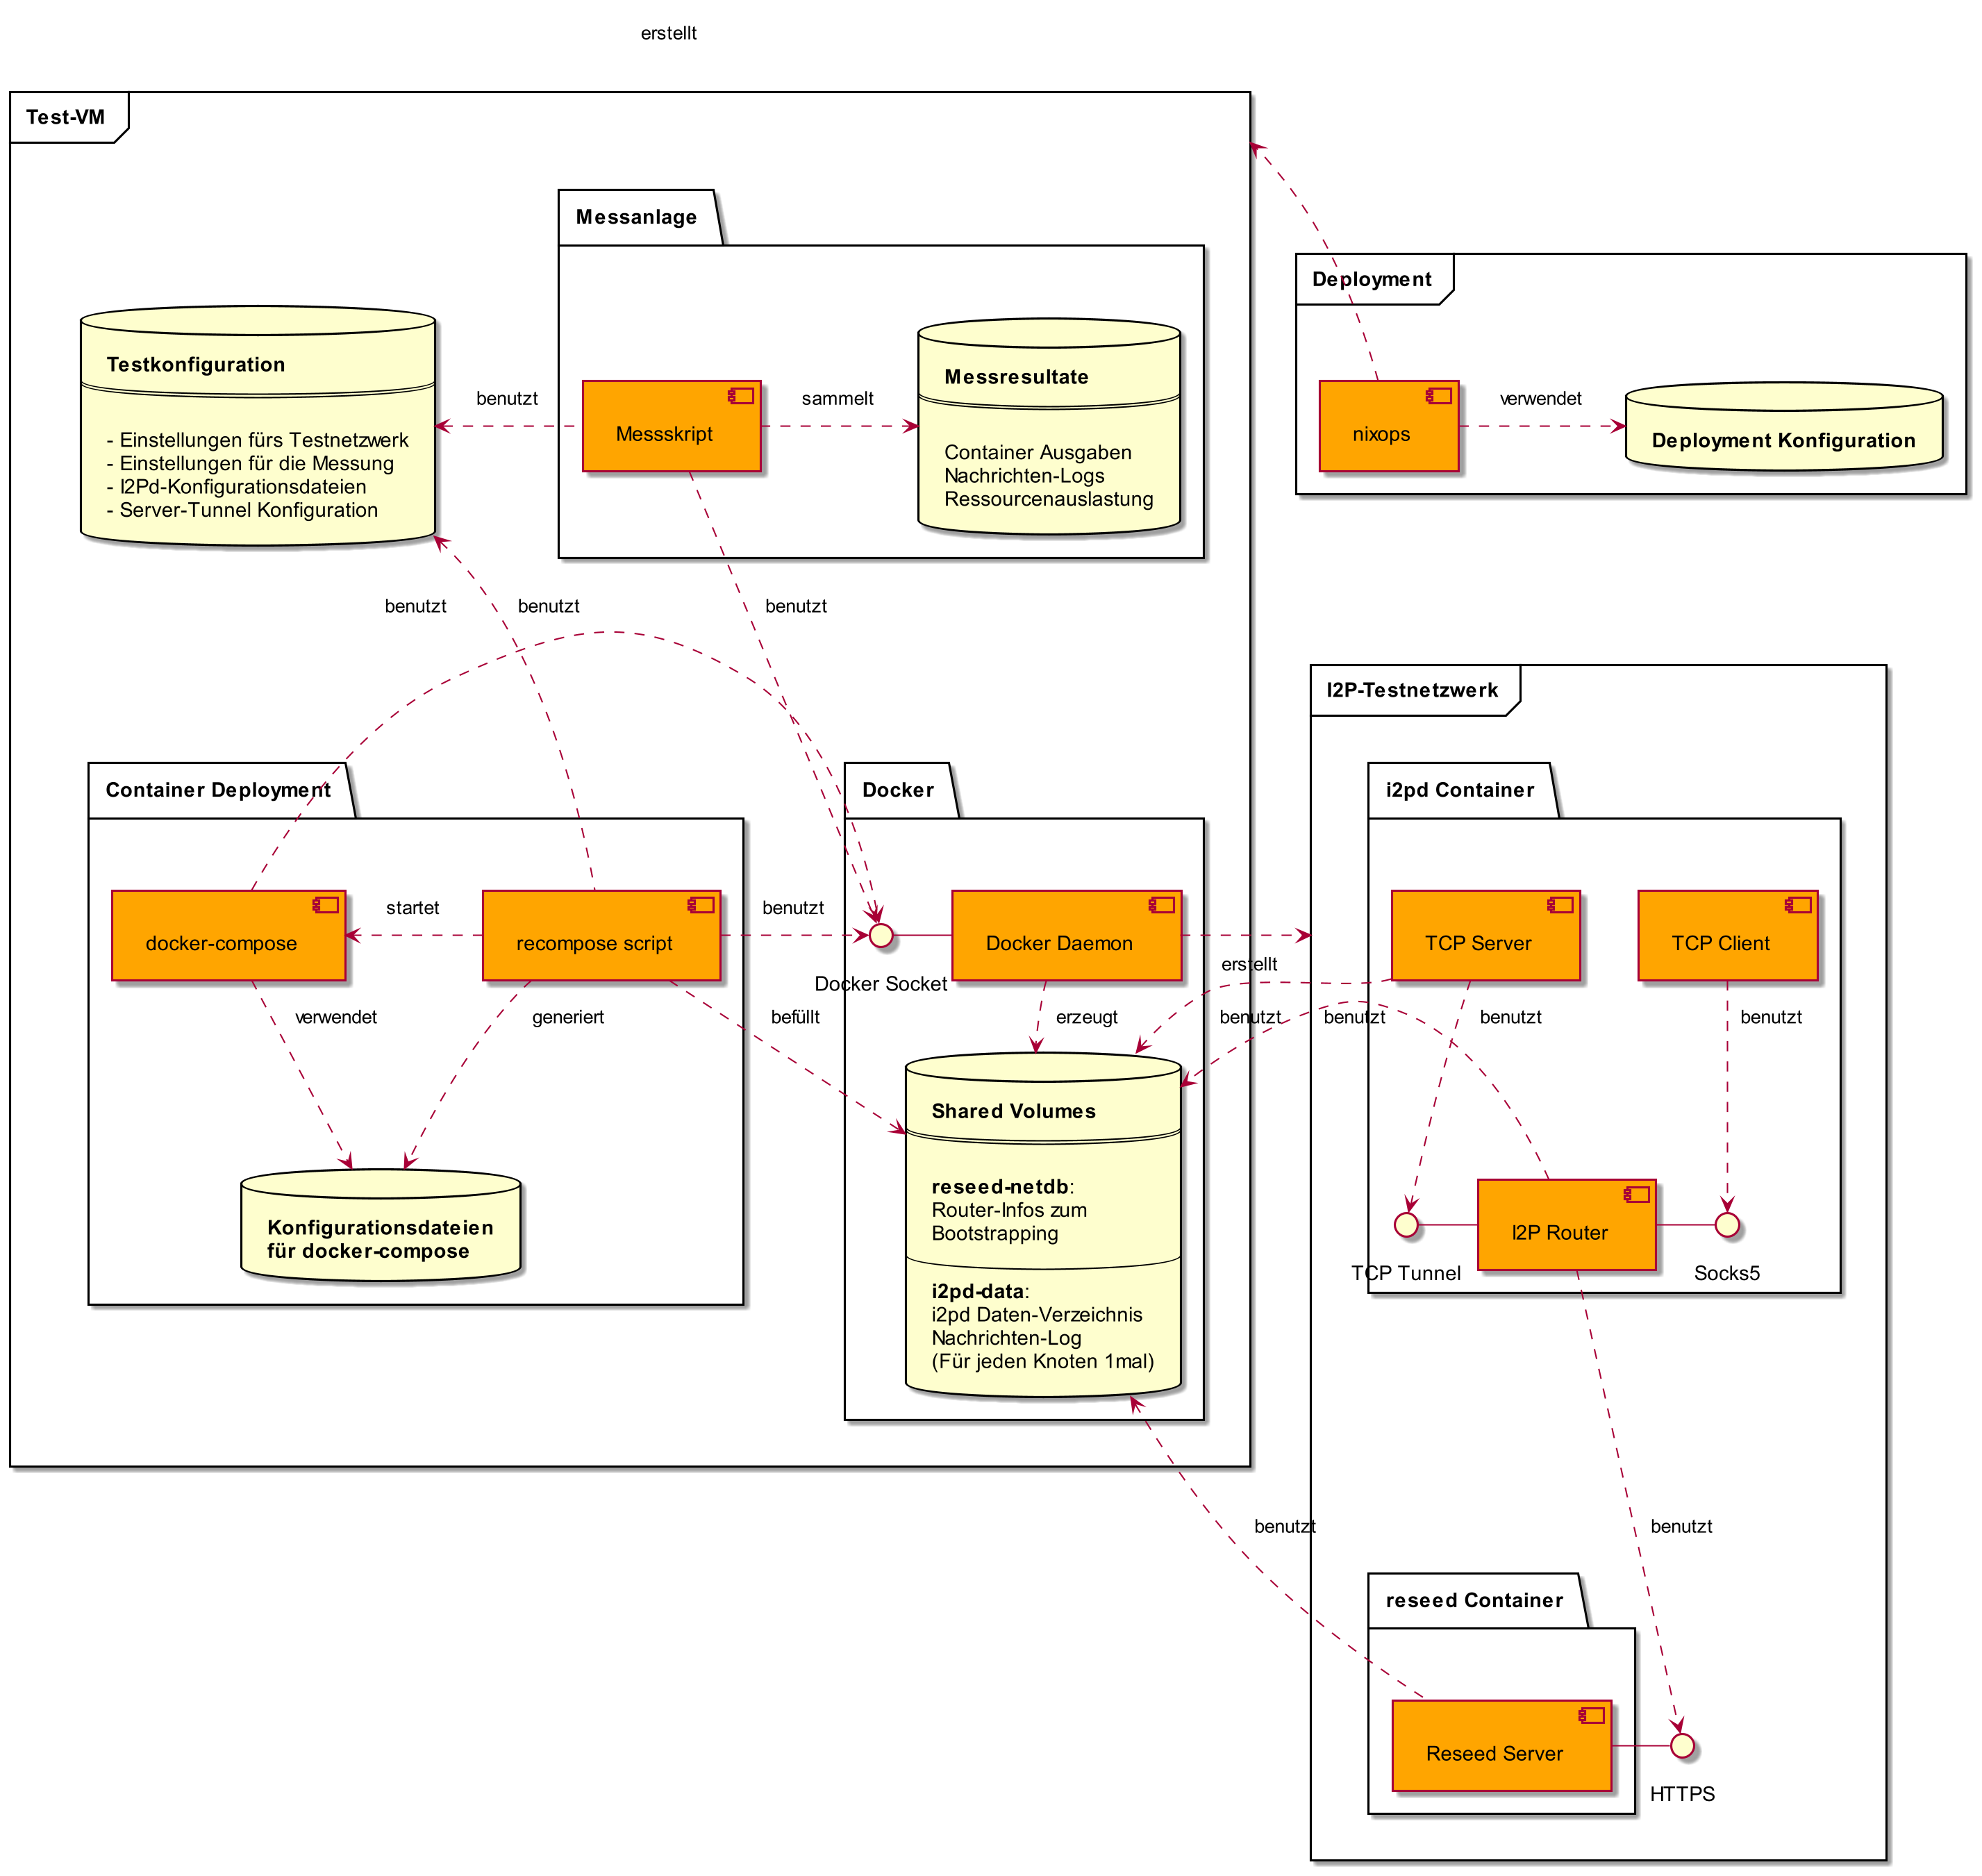
\includegraphics[height=0.85\textwidth]{include/uml/componentDiagram.png}
  \caption{Architektur-Diagramm}\label{fig:architektur-diagramm}
\end{figure*}
\end{landscape}% Landscape page


\section{Komponentendesign}

\subsection{Deployment der Test-VM}

NixOps erlaubt es eine NixOS-Systemkonfiguration auf diverse Arten von Maschinen zu deployen.

\subsection{Konfiguration}

Die Konfiguration für

\subsection{Recompose-Skript}

Das Recompose-Skript ist dafür verantwortlich das Docker-Netzwerk aufzubauen und zu managen.

Als wichtigster Punkt wird hier der 



\subsection{Deployment von der Container}

Da ich bereits NixOps zum deployment der Container verwendet habe, schien es naheliegend die NixOS-Container Technologie zu verwenden.

Jedoch bin ich mit diesem Ansatz an mehreren Stellen an Grenzen gestossen.

Als erstes traten Probleme mit der Netzwerkkonfiguration. Die NixOS-Container implementation scheinte die 

• Erst Probleme mit der Netzwerkkonfiguration
• Probleme mit Docker-Kompatibilität
• Skaliert nicht auf mehr als ein paar dutzend Container. Zu viel
RAM benötigt lediglich zum Berechnen der verschiedenen
Container-Konfigurationen.

Es hat 

Anfangs wurde auf ein Ansatz mit 


\subsection{Skalierung der i2pd-Container}

Der erste Lösungsansatz mit NixOS-Containern hat sich als ungeeignet herausgestellt. \seereq{TSCL}

Dieser Ansatz wurde verworfen, weil dies dazu geführt hat, das die i2pd-Container untereinander nicht kommunizieren konnten.

\subsection{Bootstrapping}

Die I2P-Router im öffentlichem I2P-Netzwerk können sich hier einfach an den öffentlich verfügbaren Reseeder eine \lstinline|su3|-Datei herunterladen.
Diese \lstinline|su3|-Datei beinhaltet RouterInfos. 
Diese RouterInfos beinhalten die nötigen Informationen wie public-key und Netzwerkadresse, um die Kommunikation zu starten.

Im privaten und abgeschotteten Testnetzwerk sind die öffentlichen Reseed-Server jedoch nicht erreichbar.
Deshalb muss ein anderer Weg gefunden werden das private I2P-Netzwerk zu bootstrappen.



Denn der Floodfill-Anstatz entspricht nicht unbedingt der Realität, denn die Reseeder-Knoten können liefern nicht allen I2P-Routern dieselbe Liste an Peers.

Auch kann die Konfiguration des Reseeders eine wichtige Rolle spielen, denn dieser bestimmt mit der Liste an Peers die er den I2P-Routern liefert den Konnektivitätsgrad der Knoten.


\subsection{Konfiguration}

Die Konfiguration des Teststands kann mittels einer json-Konfigurationsdatei einfach angepasst werden.
Diese kann, falls nötig einfach von verschiedenen Orten gelesen werden.

\subsection{Resultate zurücklesen}

Just read logs? Use some Docker cp magic?

\section{Umsetzung / Programmierung}

Der Komplette Quellcode für das Deployment der Test-VM, die Erstellung des Testnetzwerk's und die Messanlage ist im folgenden Repository zu finden:

\url{https://codeberg.org/mkuettel/i2p-testnet}.

\section{Test-VM}

Die Test-VM wurde so umgesetzt, das diese mittels nixops deployed werden kann.

\section{1. Lösungsansatz: NixOS-Container}

NixOS erlaubt es deklarativ Container zu definieren.

% \begin{lstlisting*}[language=nix,label=src:nixos-container,caption=Beispiel wie Nixos Container definiert werden können]
%
%     boot.enableContainers = true;
%     containers = {
%         "container1" = {
%             config = { config, pkgs, ... }:
%                 {
%                     # NixOS system configuration for this container
%                     services.httpd.enable = true;
%                 }
%             # more container settings ... 
%         };
%         # "container2" .... 
%     }
% \end{lstlisting*}

Wichtig dabei ist, dass es sich hierbei nicht um einen Docker-Container, sondern um NixOS-Container handelt.
Im Hintergrund brauchen jedoch beide Container-Arten die gleichen Linux-Kernel-Features (namespaces, cgroups, ... ).


Siehe \lstinline|containers.nix| in der \lstinline|i2p-testnet| Repository für die Effektive implementation

\subsection{Bootstrapping}

Da das Testnetzwerk

\subsubsection{Reseed-Server}

Dieser Ansatz hat den Vorteil, das so das Testnetzwerk schnell aufgebaut werden kann.

Die \lstinline|i2pd|-Implementation beinhaltet selber keinen 

Die Go-Implementation dieses Reseed-Servers ist hier zu finden:

\url{https://codeberg.org/diva.exchange/i2p-tools}

Diese Version basiert auf der folgenden GitHub version:

\url{https://github.com/MDrollette/i2p-tools}

\subsubsection{Ablauf}

Der Bootstrapping-Vorgang im Testnetzwerk wird wie folgt abgehandelt (vgl. mit Abbildung~\fullref{fig:bootstrap-diagram}):

\begin{enumerate}
    \item Erstellen der Container für den Reseed-Sever und den I2P-Knoten
    \item Der Reseed-Server erstellt die nötigen Schlüssel und Zertifikate, um einerseits später den HTTPS-Reseed-Server zu starten und andererseits die su3-Dateien zu signieren.
    \item Der Reseed-Server-Container fängt an zu warten bis er alle RouterInfo's von allen I2P-Knoten erhalten hat
    \item Die I2P-Router werden kurzzeitig gestartet, bis diese Ihre RouterInfo Datei erstellen. Die I2P-Router werden anschliessend wieder gestoppt, da der Reseed-Server im Moment noch nicht in Betrieb ist, da ihm die RouterInfos noch fehlen.
    \item Die I2P-Knoten-Container warten anschliessend bis der HTTPS-Reseed-Server verfügbar ist.
    \item Auf der Test-VM kopiert ein Hintergrund-Job alle RouterInfos vom I2P-Container in die NetDb des Reseed-Server-Containers.
    \item Nach kurzer Zeit hat der Reseed-Server-Container alle benötigten RouterInfos. Nun generiert dieser die su3-Datei aus den RouterInfos und startet anschliessend nun effektiv den HTTPS-Reseed-Server.
    \item Die I2P-Knoten-Container können nun den HTTPS-Reseed-Server erreichen und somit wird der I2P-Router gestartet.
    \item Die I2P-Router laden nun die su3-Datei herunter und können so die anderen Knoten ausfindig machen und Ihre Arbeit starten.
\end{enumerate}

Welche Reseeder ein I2P-Router anfragt, kann mittels der \lstinline|i2pd|-Konfigurationsoption \lstinline|urls| festgelegt werden.


\clearpage
\begin{landscape}% Landscape page
\begin{figure*}[ht]
  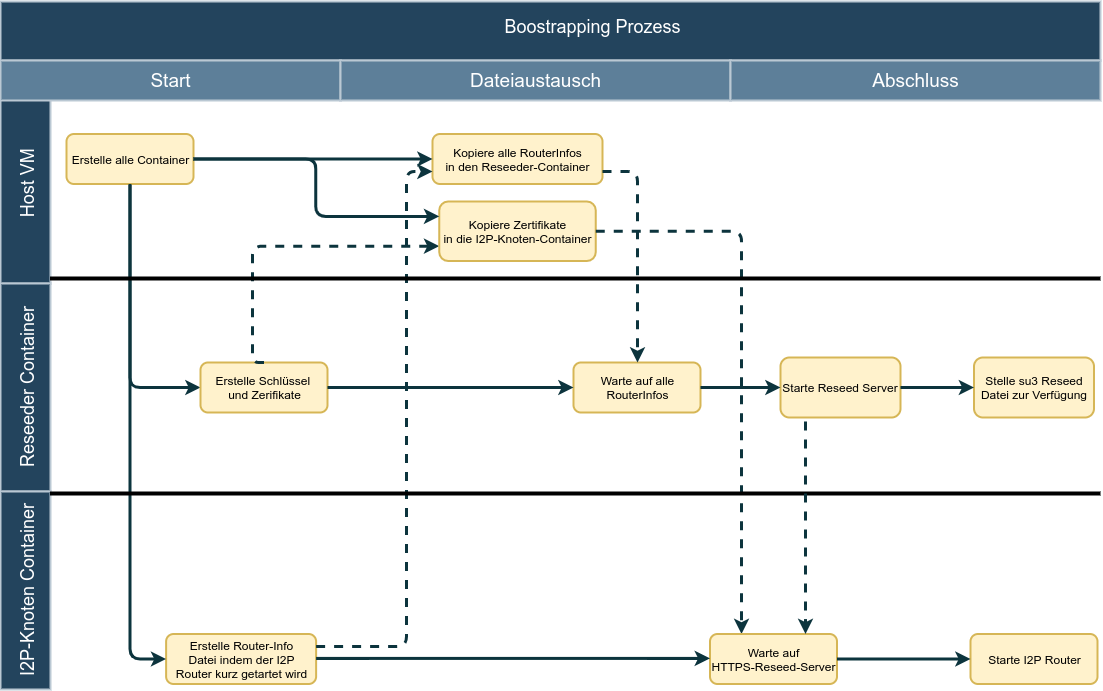
\includegraphics[height=0.85\textwidth]{bootstrap-diagram.png}
  \caption{Der Bootstrapping Prozess}\label{fig:bootstrap-diagram}
\end{figure*}
\end{landscape}% Landscape page


\subsection{Reproduzierbarkeit}

* Nix
* Pinning
    
\cite{noauthor_nixops_nodate-5}


\subsection{Isolieren}

Während unserer Tests wollen wir nur Traffic unserer eigenen Knoten im Netzwerk 

docker-compose respektive docker hat die option ein internes Netzwerk zu erstellen.

\subsubsection{Abgrenzen vom Haupt-Netzwerk}

Die Konfigurationsoption \lstinline|netid| erlaubt es die Netzwerknummer zu definieren.
Beim realen I2P-Netzwerk ist diese standardmässig auf \lstinline|2| gesetzt.

VM / Container, Konfigurationsoption \lstinline|nat|

Nix für container scheint nicht so gut zu funktionieren

Weil:

Das Builder der systemkonfigurationen inkl. der container getestet mit 100 konnte nicht durchlaufen da nix viel memory braucht (ich habe nach 16GB und 20min warten aufgehört da mein Laptop am swappen war)
Fehlerhafte netzwerkkonfiguration by default, falsche routen und ip konfigurationen (fehlende definition der netzwerkmaske)
Container selber sind unnötig gross


\subsection{I2Pd-Container}

Hauptsächlich wird in diesem Container der \lstinline|i2pd|-Prozess ausgeführt.
Um andere Knoten zu kontaktieren zu können muss dieser zu Beginn den Reseed-Container anfragen nach einer Liste von RouterInfos.

Der TCP-Client und TCP-Server sind ebenfalls in diesem Container angesiedelt.
Dies verletzt zwar das Prinzip, dass man nur einen Prozess in einem Docker-Container ausführen sollte,
jedoch ist das Ziel hiermit Messungenauigkeiten durch das Netzwerk, sowie die Netzwerkkonfiguration zu vereinfachen.

\subsection{Addressbuch}

%TODO: add to state of the art?

Standardmässig wird jeder i2pd-Destination eine b32-Adresse gegeben.
Diese Adresse wird abgeleitet vom Public-Key der generierten Destination.

Diese ist eine 52-Zeichen-lange aus kleinbuchstaben und zahlen bestehender Name um eine Destination zu adressieren. (z.b. \lstinline|b2cdodoyqg5v6go56bkaevvw777e2wyiflqh6zyyyxugy4cqlzuq.i2p|)

Zudem hat diese die Endung \lstinline|.i2p| damit klar ist, das dieser Name innerhalb des Overlaynetzwerks aufgelöst werden muss.

Diese ist jedoch nicht einfach zu handhaben und anstatt es ist einfacher die Knoten direkt anhand ihrer Nummer zu adressieren. Damit kann das Messskript vereinfacht werden, da es dieses dann nicht die 

Auch wird die Auswertung damit vereinfacht weil, der TCP-Client den verwendeten Namen des TCP-Servers auch in die Nachricht hineinpackt und der TCP-Server diesen als Messausgabe abspeichert.

Es wird beim Startvorgang des Netzwerks für jede erstellte destination für den TCP-Server ein Adressbucheintrag erstellt. Dieses Adressbuch ist eine einfache CSV-Datei wird wird 
im Bootstrapvorgang an alle Knoten verteilt.

Im falle von acht Knoten im Netzwerk sieht diese Datei beispielsweise so aus:

\begin{lstlisting}
tcpsrv-1.i2p,b2cdodoyqg5v6go56bkaevvw777e2wyiflqh6zyyyxugy4cqlzuq
tcpsrv-2.i2p,r6axddltht76mrtp5lrxtdxncilhgp7bcajkqtsj7l7fmoebgs3a
tcpsrv-3.i2p,ddhznqpxtgac7qa6yg6uzfpd55xoa2zfc4dwg4rh4qucx7veswlq
tcpsrv-4.i2p,3tyncnh7j4akqirrbdi4ek7nlysqmuvyav3ix326vwixvgoviz3q
tcpsrv-5.i2p,xj3qduyqur54v3mjgsxn6xa56q2ojyysf5n3bonpxyfxy5trnoja
tcpsrv-6.i2p,pt64eojrsvrp5w5izgwlide7j6vuw5td6g2pfrkurwsnmb4i7q2q
tcpsrv-7.i2p,aat6wqge3o7k2nabpwxrcu2vbbiydf3mj6n5k2zrrtozkrrpyfoa
tcpsrv-8.i2p,4wm4pqautqqb3a6yw3xif4zgwwu4v5tvpwv6onha27p5pkcqqepq
\end{lstlisting}

In der ersten Spalte ist der vereinfachte Name anzugeben und in der Zweiten Spalte die b32-Addresse, jedoch ohne die Endung \lstinline|.i2p|

\subsection{Der I2Pd-Prozess}

\subsubsection{TCP Server Tunnel}

Diese Tunnel-Konfiguration führt dazu, dass I2P eine neue Destination mit einer .b32-Addresse erstellt.

Mit der folgenden Tunnel-Konfigurations-Datei wird der \lstinline|i2pd| konfiguriert, um einen TCP-Server-Tunnel zur Verfügung zu stellen:
\begin{lstlisting}
# serve some tcp service to others in the network
[tcp-in]
type = server
host = 127.0.0.1
port = 2323
keys = tcp-in.dat
gzip = false
enableuniquellocal = true
\end{lstlisting}

Hierbei gilt es zu beachten, das die Schlüssel angegeben mit der \lstinline|keys|-Option, beim Aufstarten generiert werden.
Auch wurde mittels der Option \lstinline|gzip| die Komprimierung-Deaktiviert, damit auch wirklich die richtigen Nachrichten-Grössen übermittelt werden.
Die Option\lstinline|enableuniquellocal| wurde noch aktiviert, um die Auswertung zu vereinfachen. Denn diese führt dazu das der TCP-Server nicht immer dieselbe Ausgangsadresse \lstinline|127.0.0.1| bekommt, sondern je nach Sender der Nachricht eine andere \lstinline|127.0.0.0/8|-Adresse anhand der ersten Bytes des Public-Keys erhält.

%TODO: Reference config, especiallfor for enableuniquellocal.


\subsubsection{Socks5-Proxy für den TCP-Client}

Dieser Socks5-Proxy ist der Gateway um innerhalb des I2P-Overlaynetzwerk zu kommunizieren.

Der folgende Ausschnitt aus der \lstinline|i2pd.conf| zeigt auf wie der Socks5-Proxy konfiguriert wurde:

\begin{lstlisting}
[socksproxy]
## Uncomment and set to 'false' to disable SOCKS Proxy
enabled = true
## Address and port service will listen on, like 127.0.0.1
address = 127.0.0.1
port = 4445
\end{lstlisting}

\subsection{TCP-Server}


\subsection{TCP-Client}

Damit der TCP-Client in das I2P-Overlaynetzwerk verbinden kann muss dieser fähig sein mit einem Socks5-Proxy zu kommunizieren.



\section{Testing}

CI? most don't allow this...

have a machine to deploy to

\subsection{BATS-Tests}

Diese Tests sind im Verzeichnis \lstinline|tests/| in der \lstinline|i2p-testnet|-Repository zu finden.

Um schnell zu prüfen ob das Netzwerk korrekt konfiguriert wurde gibt es das Test-Modul \lstinline|tests/networking.bats|.

\subsection{CI für den Bericht}

Da der Bericht mit Hilfe von \LaTex umgesetzt wurde, verhält sich dieser 

\section{Benutzerhandbuch}

Dieser Abschnitt erklärt wie ein Tester selber neue Testnetzwerke erstellen, die Tests-Konfigurieren und selber

\subsection{Deployment der Test-VM}

Für genauere Anweisungen und weitere Möglichkeiten welche durch nixops geboten werden, siehe das ``NixOps User's Guide''\footnote{\url{https://releases.nixos.org/nixops/nixops-1.5/manual/manual.html}}.


\subsection{Konfiguration einer Messung}

\subsection{Ausführen einer Messung}


\chapter{Evaluation und Validation}
\label{ch:Eval}

% Auswertung und Interpretation der Ergebnisse. Nachweis, dass die Ziele erreicht wurden, oder
% warum welche nicht erreicht wurden.

Quantitative Auswertung

\section{Validation der Testumgebung}

Um Aussagen machen zu können über das Testnetzwerk muss erst sichergestellt werden, dass die Messwerte Sinn ergeben.
Deshalb wurden erste Tests durchgeführt, um zu prüfen, ob die Testumgebung auch richtig funktioniert.

Diese Messungen bieten auch eine Basis und einen Referenzpunkt für die weiteren Messungen.

\subsection{Wiederholbarkeit von Messungen}

Als Teil dieser Messung wird erst ein Netzwerk mit 8 Knoten getestet und die Latenz von 1000 Nachrichten gemessen.
Alle Knoten haben in diesem Test keine Bandbreitenbeschränkung.
Eine Nachricht wird hier jeweils von einem zufälligen Knoten an einen anderen zufälligen Knoten versendet.
Die Konfigurierte Nachrichtengrösse wurde jeweils auf 64kB festgelegt.
Die Messung wird so festgehalten.
Anschliessend wird derselbe Test noch einmal gestartet, wobei das Testnetzwerk jedoch aber neu erstellt wird.

Grundsätzlich wird hier erwartet, dass die Messungen vergleichbar sind und ähnliche Resultate liefern.

% TODO: add measurements


Somit kann ausgesagt werden das die Messungen so gut wie möglich reproduzierbar sind \seereq{TREP}.


\subsection{Gleichbleibende Latenz bei Skalierung des Netzwerks}

Um sicherzustellen, dass kein Fehler beispielsweise im implementieren Testnetzwerk oder gar in der i2pd-Software aufzufinden ist, wird diese Messung zu Validierungszwecken durchgeführt.

Alle Knoten haben in diesem Test keine Bandbreitenbeschränkung.
Eine Nachricht wird hier jeweils von einem zufälligen Knoten an einen anderen zufälligen Knoten versendet.
Die Konfigurierte Nachrichtengrösse wurde jeweils auf 64kB festgelegt.
Die Messung wird so festgehalten.

Anschliessend wird die gleiche Messung noch einmal gestartet.
Jedoch wird die Anzahl Knoten im Testnetzwerk jeweils verdoppelt.

Es wird angenommen, dass sich die Latenz der Nachrichten im Netzwerk nicht hier verändert.
Dies mag auf den ersten Blick der Hyptothese wiedersprechen, jedoch gilt es zu beachten, dass hier alle Knoten dieselbe Bandbreitenbeschränkung haben.
%TODO: ref hypothese



\section{}



\section{Vergleich mit Anforderungen}
\label{sec:VergleichAnforderungen}
% TODO Vergleich mit Anforderungen Soll<->Ist

\seereq{}



\section{Technische Aspekte}
% TODO Evaluation der verwendeten Hilfsmittel

\section{Vorgehen}
% TODO Evaluation der verwendeten Arbeitsprozesse


% !TEX root = BA-Bericht.tex
\chapter{Ausblick}
\label{ch:Ausblick}
$% umbenennen Abschluss

% Reflexion der eigenen Arbeit, ungelöste Probleme, weitere Ideen.


\section{Projekt Fazit}
% TODO Das Fazit des Projektes, auch eine Unterteilung in \subsection mit persönlichem und Projektfazit ist möglich

Diese Arbeit konnte mit dem erstellen eines I2P-Testnetzwerks nun einen Grundstein legen für weitere Untersuchungen.


\section{Persönliches Fazit}

Ich finde dies und das....

\section{Ausblick}
% TODO Was ist für Folgeprojekte wichtig, welche Lehren können gezogen werden, was sind noch offene Fragen?

Diese Arbeit 

\begin{itemize}
    \item Es gibt andere Möglichkeiten Nachrichten über das I2P-Netzwerk zu versenden.
    Unter anderem gibt es das SAM-Protokoll.  Es könnte möglich sein bessere Performance mit diesem Protokoll zu erreichen anstatt einen SOCKS5 oder HTTP-Proxy zu verwenden. \cite{noauthor_sam_nodate}
    Der Nachteil bestände jedoch darin, dass die darüberliegende Datenhaltungsschicht dieses Protokoll implementieren müsste und fest an I2P gekoppelt wäre.
    \item Horizontal Skalieren
    \item Cloves / Garlic-Routing
    \item Peer-Profiling
\end{itemize}


\newpage

\pagenumbering{Roman}

\appendix
% Verhindert das Einfügen von Kapiteltitel kleiner als \chapter
\addtocontents{toc}{\protect\setcounter{tocdepth}{0}}

\printglossary

\listoffigures

\listoftables

\listofmyequations \pagebreak

\printbibliography

% !TEX root = BA-Bericht.tex
 % TODO Anhänge anfügen
% Wir haben dies jeweils über \chapter gelöst
% \includepdf[pages=-]{PDF-ANHANG}


% TODO Anhänge anfügen
% Wir haben dies jeweils über \chapter gelöst
% \includepdf[pages=-]{PDF-ANHANG}


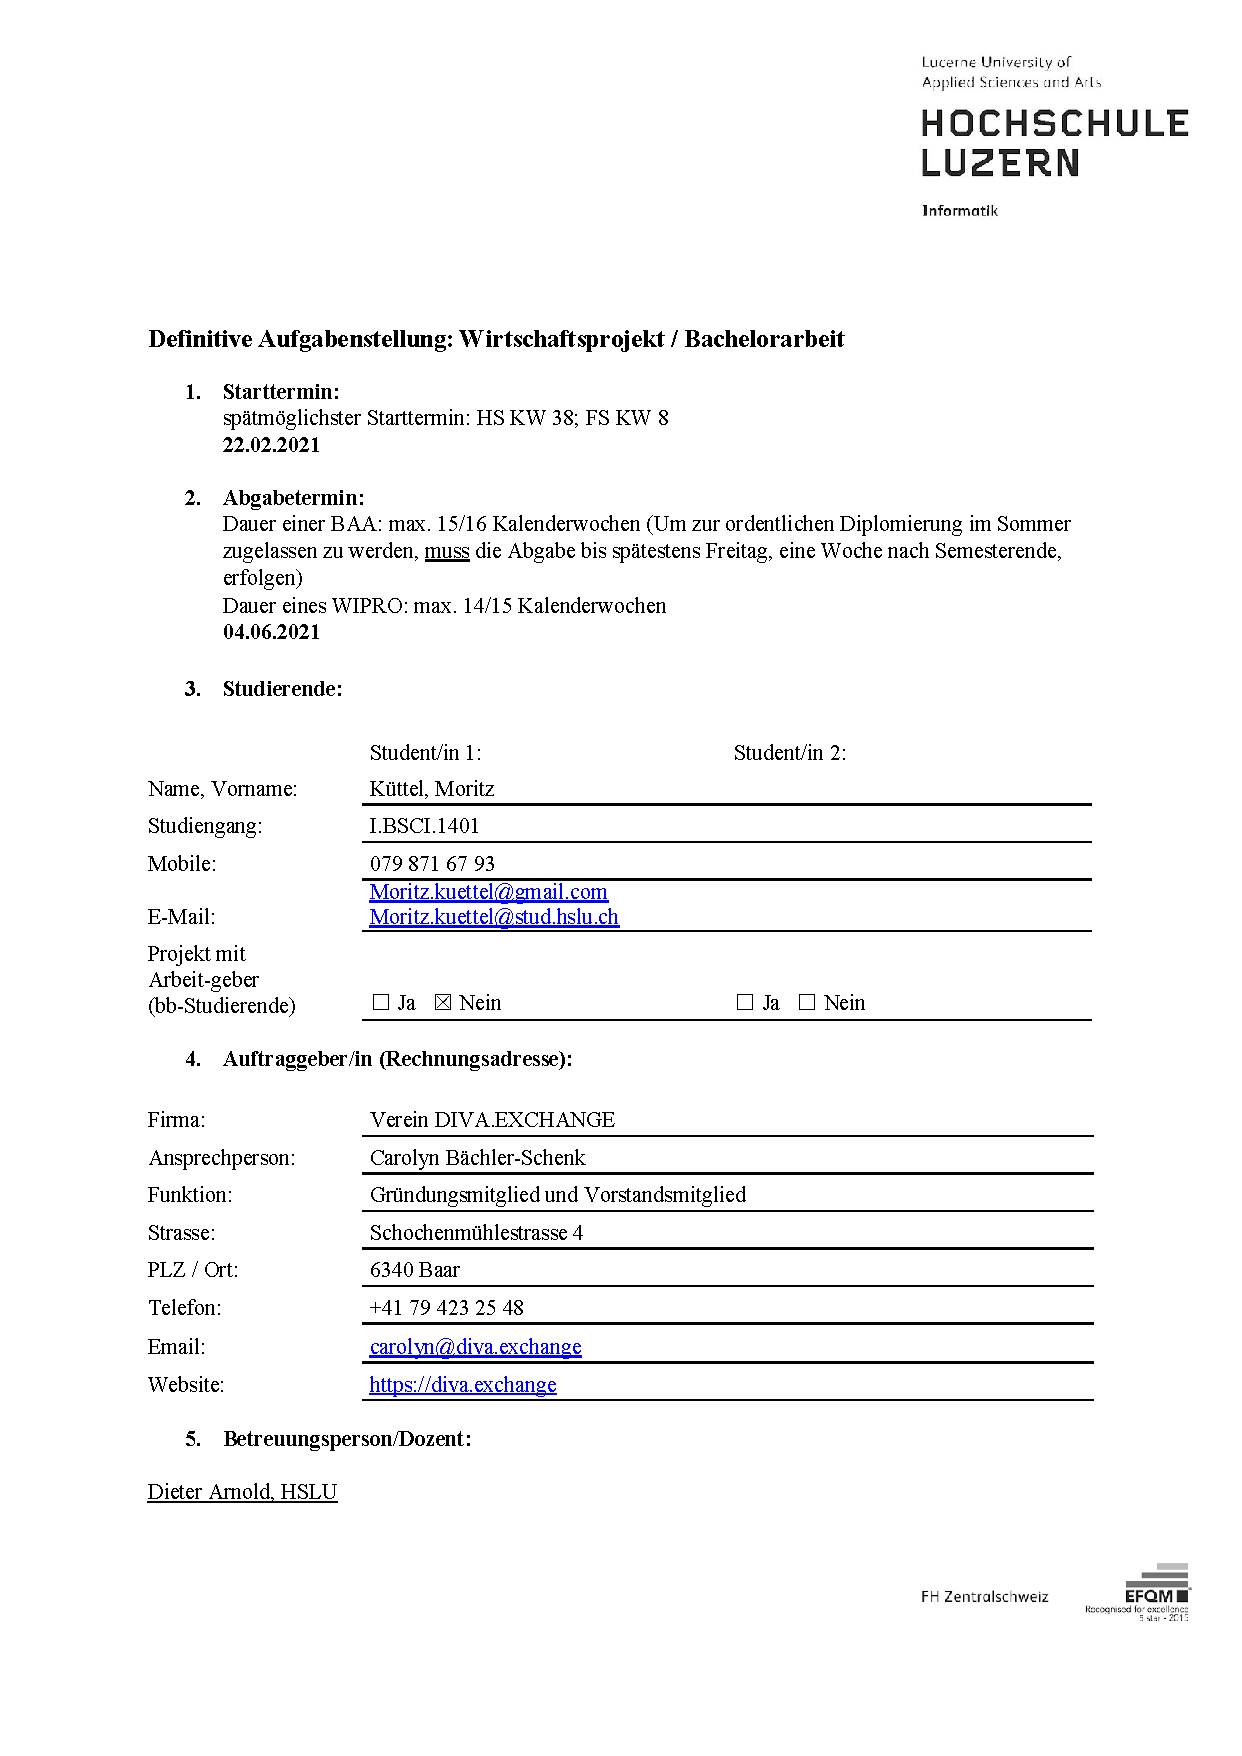
\includepdf[
     addtotoc={1,chapter,0,Aufgabenstellung,ch:aufgabenstellung},
     pages=-
     ]{include/129_BAA_Aufgabenstellung.pdf}\label{ch:assignment}

\chapter{Resultate}\label{ch:resultate}

Die folgende Tabelle~\fullref{tab:resultate} beschreibt Resultate und Unterresultate die während dieser Bachelorarbeit erarbeitet werden sollen.
Diese Tabelle wurde zu Beginn des Projekts zusammengestellt anhand der Anforderungen im Abschnitt~\ref{sub:Anforderungen}.
Sie wurde aus Planungsgründen erstellt, um etwa einschätzen zu können, wie viel Aufwand welche Teile der Arbeit mit sich bringen und den Umfang abzugrenzen.
Jedes Resultat hat einen eindeutigen Identifier in  der Spalte ''Nr'' aufgelistet.
Die Spalte ``Anforderung'' bezieht sich darauf, welche Anforderungen für das jeweilige Resultat massgebend sind.
In der letzten Spalte ''Geschätzter Arbeitsaufwand'', wurde zu beginn des Projekts abgeschätzt, wie viel Arbeitsaufwand (in Stunden) das Resultat verursacht.

\begin{longtable}{p{0.8cm} l p{3.5cm} p{2cm}}
    \toprule
    \bfseries Nr & \bfseries Resultat & \bfseries Anforderung& \multicolumn{1}{p{3cm}}{\bfseries Geschätzter Arbeitsaufwand} \\
    \midrule \endhead
    D            & \textbf{Dokumentation}                                       & \reqref{DOCS} & \textbf{Total 44h}  \\
    \midrule                                                               
    D.1          & \; Dokumenten Layout                                &       & 8h   \\
    D.2          & \; Aufbau des Berichts                              &       & 4h   \\
    D.3          & \; Titelseite                                       &       & 2h   \\
    D.4          & \; Zusammenfassung / Abstract                       &       & 2h   \\
    D.5          & \; Einleitung                                       &       & 4h   \\
    D.6          & \; Beschreibung Motivation / Problem                &       & 2h   \\
    D.7          & \; Beschreibung der Aufgabenstellung                &       & 2h   \\
    D.8          & \; Beschreibung der Ziele / Vision                  &       & 1h   \\
    D.9          & \; Fragestellungen / Hypothesen                     &       & 2h   \\
    D.11         & \; Reflektion / Fazit                               &       & 3h   \\
    D.12         & \; Persönliches Projektfazit                        &       & 1h   \\
    D.13         & \; Ausblick                                         &       & 4h   \\
    D.14         & \; Anhang                                           &       & 3h   \\
    D.15         & \; Zwischenpräsentation                             & \reqref{PRES}  & 6h  \\
    \midrule                                                               
    R            & \textbf{Recherche}                                           & \reqref{SDTF} \reqref{DOCS}  & \textbf{Total 40h} \\
    \midrule                                                               
    R.1          & \; Literatur sammeln (Recherche)                    &       & 12h  \\
    R.2          & \; Bibliographie erstellen                          &       &  4h  \\
    R.3          & \; P2P Networks                                     &       &  2h  \\
    R.3.1        & \;   - Latenz / Bandbreite / Performanz             &       &  2h  \\
    R.4          & \; Beschreibung I2P                                 &       & 10h  \\
    R.4.1        & \; -- Begrifflichkeiten                              &       &  4h  \\
    R.4.2        & \; -- Funktionsweise                                 &       &  2h  \\
    R.4.3        & \; -- Bandbreite                                     &       &  2h  \\
    R.4.4        & \; -- Latenz                                         &       &  2h  \\
    R.5          & \; Deployment von Testnetzwerken                    &       &  4h  \\
    R.6          & \; Beschreibung der wissenschaftlichen Methode      &       &  2h  \\
    R.7          & \; Metriken für die Auswertung                      & \reqref{TPER} \reqref{TISO} \reqref{TREP}  &  6h  \\
    \midrule                                                               
    K            & \textbf{Testkonzept          }                               & \reqref{TKON} \reqref{DOCS}  & \textbf{Total 46h}  \\
    \midrule                                                               
    K.1          & \; Beschreibung Ideen / Konzepte                    &       &  4h  \\
    K.2          & \; Anforderungen an den Teststand                   &       &  4h  \\
    K.3          & \; Teststrategie                                    &       &  4h  \\
    K.4          & \; Architektur Teststand                            &       &  4h  \\
    K.5          & \; Komponentendiagramm                              &       &  2h  \\
    K.6          & \; Beschreibung was gemessen werden soll            &       &  8h  \\
    K.7.1        & \; -- Bandbreite                                     & \reqref{TLIM} &  2h  \\
    K.7.1        & \; -- Anzahl Tunnels                                 & \reqref{TCNF}    &  2h  \\
    K.7.1        & \; -- Latenz von Nachrichten                         & \reqref{TLAT}    &  2h  \\
    K.7.1        & \; -- Ressourcenauslastung eines Knotens             & \reqref{TPER}    &  2h  \\
    K.8          & \; Beschreibung wie gemessen wird                   &       & 10h  \\
    K.8.1        & \; -- Isolation des Netzwerks                        & \reqref{TISO}    &  2h  \\
    K.8.1        & \; -- Verschiedene Netzwerksegmente                  & \reqref{TISO}    &  2h  \\
    K.8.2        & \; -- Latenz                                         & \reqref{TLAT}    &  2h  \\
    K.8.3        & \; -- Bandbreite                                     & \reqref{TLIM}      &  2h  \\
    K.8.4        & \; -- Konfigurationsmöglichkeiten                    & \reqref{TCNF} &  2h  \\
    K.9.5        & \; \glsname{ci}                                     & \reqref{TVRS} &  6h  \\
    K.9.6        & \; Beschreibung der Auswertungsmethode              &               &  4h  \\
    \midrule                                                               
    I            & \textbf{Teststand Design und Implementation}                 & \reqref{TINF} \reqref{DOCS} & \textbf{Total 124h} \\
    \midrule
    I.1          & \; Software Design                                  &       &  16h \\
    I.1          & \; Implementation                                   &       &  72h \\
    I.2.1        & \; -- Deployment des Testnetzwerkes                  & \reqref{TVRS} \reqref{TPER} &  8h \\
    I.2.2        & \; -- Netzwerksegmentierung                          & \reqref{TISO} &  8h \\
    I.2.3        & \; -- Konfigurationsmöglichkeiten                    & \reqref{TCNF} &  8h \\
    I.2.4        & \; -- Skalierung                                     & \reqref{TSCL} &  8h \\
    I.2.5        & \; -- Bandbreitenbeschränkung                        & \reqref{TLIM} &  8h \\
    I.2.6        & \; -- Reproduzierbarkeit                             & \reqref{TREP} &  8h \\
    I.2.7        & \; -- Latenzmessung                                  & \reqref{TLAT} &  8h \\
    I.2.8        & \; -- Messung der Ressourcenauslastung               & \reqref{TPER} &  8h \\
    I.2.9        & \; -- Verschiedene Testaufbauten                     & \reqref{TVRS} &  8h \\
    I.3          & \; Test des Labors                                  &       &  24h \\
    I.4          & \; Handbuch für den Teststand                       &       &  12h \\
    I.4.1        & \; -- Installation                                   &       &   2h \\
    I.4.3        & \; -- Konfiguration                                  &       &   2h \\
    I.4.3        & \; -- Ausführen von Messungen                        &       &   2h \\
    I.4.3        & \; -- Beschreibung der gesammelten Messdaten         &       &   4h \\
    I.4.3        & \; -- Beispiele                                      &       &   2h \\
    \midrule                                                                        
    A            & \textbf{Messung und Auswertung}                              & \reqref{EVAL} \reqref{DOCS}   & \textbf{Total 52h}  \\
    \midrule
    A.1          & \; Sammlung an Messdaten für die Auswertung         &        &  12h  \\
    A.2          & \; Beschreibung der Auswertungsmethode              &        &   4h  \\
    A.3          & \; Auswertung der Messungen                         &                    & 20h  \\
    A.3.1        & \; -- Einfluss der Knoten auf die Latenz             & \reqref{TLAT}      &  6h  \\
    A.3.2        & \; -- Einfluss der Anzahl Verbindungen auf die Latenz& \reqref{TLAT} \reqref{TLIM} &  6h  \\
    A.3.3        & \; -- Einfluss der Bandbreite auf Latenz             & \reqref{TLAT} \reqref{TLIM} &  6h  \\
    A.3.4        & \; -- Äussere Einflüsse / Unreinheiten               & \reqref{TREP} \reqref{TISO} &  2h  \\
    A.4          & \; Verschiedene Diagramme/Grafiken                  &       &  8h  \\
    A.5          & \; Auswertung der Anforderungen an den Teststand    & \reqref{TINF} &  4h  \\
    A.6          & \; Zusammenfassung der Auswertung                   &       &  4h  \\
    \midrule                                                               
    P            & \textbf{Project Management Dokumentation}                    & \reqref{DOCS} \reqref{ITER}  &  \textbf{Total 54h}  \\
    \midrule
    P.1          & \; Beschreibung Projektorganisation                 &       &  1h  \\
    P.3          & \; Projektmanagement Methode                        &       &  2h  \\
    P.2          & \; Beschreibung Projektumfang                       &       &  2h  \\
    P.4          & \; Projektplanung                                   &       &  8h  \\
    P.5          & \; Liste von Requirements                           &       &  4h  \\
    P.6          & \; Liste von Resultaten                             &       &  4h  \\
    P.9          & \; Arbeitsjournal                                   &       &  4h  \\
    P.10         & \; Meeting-Protokolle und Notizen                   &       & 29h  \\
    \midrule                                                               
                 & \bfseries  Geschätzter Arbeitsaufwand               & \textbf{Total} & \bfseries 360h \\
    \midrule
    \bottomrule
    \caption{Resultate}
    \label{tab:resultate}
\end{longtable}

% \chapter{Meeting-Notizen}
% \label{ch:meetingnotes}
%
%
% \includepdf[
%     addtotoc={1,section,1,Notizen  Kick-Off-Meeting 24.02.2021,sec:meeting_24_02_2021},
%     pages=-
% ]{Meetings/24-02-2021.pdf}
%
% \includepdf[
%     addtotoc={1,section,1,Meeting-Notizen 26.02.2021,sec:meeting_26_02_2021},
%     pages=-
% ]{Meetings/26-02-2021.pdf}
%
% \includepdf[
%     addtotoc={1,section,1,Meeting-Notizen 03.03.2021 9:30,sec:meeting_03_03_2021},
%     pages=-
% ]{Meetings/03-03-2021.pdf}
%
%
% \includepdf[
%     addtotoc={1,section,1,Meeting-Notizen 03.03.2021 14:00,sec:meeting_03_03_2021},
%     pages=-
% ]{Meetings/03-03-2021-1400.pdf}
%
%
% \includepdf[
%     addtotoc={1,section,1,Meeting-Notizen 05.03.2021,sec:meeting_05_03_2021},
%     pages=-
% ]{Meetings/05-03-2021.pdf}
%
%
% \includepdf[
%     addtotoc={1,section,1,Meeting-Notizen 10.03.2021,sec:meeting_10_03_2021},
%     pages=-
% ]{Meetings/10-03-2021.pdf}
%
% \includepdf[
%     addtotoc={1,section,1,Meeting-Notizen 12.03.2021,sec:meeting_12_03_2021},
%     pages=-
% ]{Meetings/12-03-2021.pdf}
%
% \includepdf[
%     addtotoc={1,section,1,Meeting-Notizen 24.03.2021,sec:meeting_24_03_2021},
%     pages=-
% ]{Meetings/24-03-2021.pdf}
%
% \includepdf[
%     addtotoc={1,section,1,Meeting-Notizen 31.03.2021,sec:meeting_31_03_2021},
%     pages=-
% ]{Meetings/31-03-2021.pdf}
%
% \includepdf[
%     addtotoc={1,section,1,Meeting-Notizen 14.04.2021,sec:meeting_14_04_2021},
%     pages=-
% ]{Meetings/14-04-2021.pdf}
%
% \includepdf[
%     addtotoc={1,section,1,Zwischenpräsentation 21.04.2021,sec:meeting_21_04_2021},
%     pages=-
% ]{Meetings/21-04-2021.pdf}


\clearpage% Flush earlier floats (otherwise order might not be correct)
\begin{landscape}% Landscape page
\chapter{Journal}
\label{sec:journal}

    Die folgende Tabelle \fullref{tab:journal} listet die geleisteten Stunden für diese Bachelorarbeit auf. Jede Zeile beinhaltet einen Task und ist unter umständen mit einem oder mehreren Issues auf codeberg.org verbunden.

    \scriptsize

    \begin{longtable}{r l r r r p{2.2cm} p{4.5cm} p{4.5cm} }
        \toprule
        \bfseries Datum & \bfseries Ort & \bfseries Von &
        \bfseries Bis & \bfseries Stunden &
        \bfseries Issue \# & \bfseries Task & \bfseries Notizen \\
        \midrule

        \endhead{}

        \csvreader[
            late after line=\\\midrule,
            late after last line=\\\midrule,
        ]{include/journal.csv}{}
        {\csvlinetotablerow}

       \csvreader[
           head to column names,
           late after line=\\\midrule,
           late after last line=\\\bottomrule,
         ]{include/journal-total-hours.csv}{}
         {& & \bfseries Total (Ist)  & \bfseries hours & \Hours{} \\
          & & \bfseries Total (Soll) & \bfseries hours & 360:00
         }
        \caption{Journal}\label{tab:journal}
    \end{longtable}

\end{landscape}
\clearpage% Flush page



% \chapter{Other Markdown stuff?}
% \label{ch:OtherMarkdownStuff}
% \markdownInput[shiftHeadings=1]{include/somwhere/something.md}



\end{document}
